% % % % % % % % % % % % % % 
%
%	U.S. Macro and Markets Dashboard
%	Brian W. Dew (brianwdew@gmail.com)
%	As of: April 26, 2017
%
% % % % % % % % % % % % % %
	\documentclass{report}

%
% Packages
%
	\usepackage[right=1.0in, left=0.7in, top=1.0in, bottom=1.1in]{geometry}
	\usepackage{pgfplots}
		\pgfplotsset{compat=1.14}
	\usepackage[eulergreek]{sansmath}
	\usepackage{color}
	\usepackage{amssymb}
	\usepackage[colorlinks,
  		linkcolor=cyan!50!blue,
  		filecolor=cyan!50!blue,
 		citecolor=cyan!50!blue,
 		urlcolor=cyan!50!blue,
 		linktoc=all]{hyperref}

%
% Sans serif font
	\renewcommand*\sfdefault{cmss}
	\renewcommand{\familydefault}{\sfdefault}

% Map
\input{safe/USAmap.tex}

\begin{document}

\noindent \noindent \color{cyan!70!blue} \footnotesize $\blacksquare$ \color{black!90} \small{Real GDP growth by state in 2016 Q1 (annual percent change)}
\vspace{5mm}

{ 		
\tikzset{set state val/.style args={#1}{#1={fill=yellow!70!green}}}
\tikzset{set state val/.list={AL, AR, CO, CT, DE, DC, HI, IN, IA, KS, MA, MN, MO, NV, NH, NJ, NM, NC, OR, TN, VA, WI, AL, CT, DC, IL, ME, MS, MO, NM, OR, SC, AK, AZ, AR, CO, DE, GA, HI, IL, IN, IA, KS, KY, LA, ME, MD, MN, MS, MO, MT, NE, NV, NJ, NM, NY, NC, ND, OH, OK, PA, RI, SC, SD, TN, VT, VA, WV, WI, WY}}
\tikzset{set state val/.style args={#1}{#1={fill=green!80!blue}}}
\tikzset{set state val/.list={AZ, CA, FL, ID, ME, MD, MI, SP, NE, OH, PA, SC, GA, HI, ID, IN, IA, KS, MD, MA, MI, SP, MT, NE, NH, NJ, NC, RI, TN, TX, VT, VA, WA, WV, AL, CA, CT, DC, FL, ID, MA, MI, SP, NH, OR, TX, UT, WA}}
\tikzset{set state val/.style args={#1}{#1={fill=red!40!orange!80}}}
\tikzset{set state val/.list={IL, MT, WV, AK, NY, OK, WY}}
\tikzset{set state val/.style args={#1}{#1={fill=blue!50!green}}}
\tikzset{set state val/.list={KY, RI, SD, AZ, CA, CO, DE, FL, KY, MN, NV, OH, PA, SD, UT, WI}}
\tikzset{set state val/.style args={#1}{#1={fill=orange!60!yellow}}}
\tikzset{set state val/.list={GA, LA, MS, NY, ND, OK, TX, UT, VT, WA, AR, LA, ND}}
\tikzset{set state val/.style args={#1}{#1={fill=red!80!black!80}}}
\tikzset{set state val/.list={AK, WY}}
%\input{test.txt}
\resizebox {\columnwidth} {!} {			
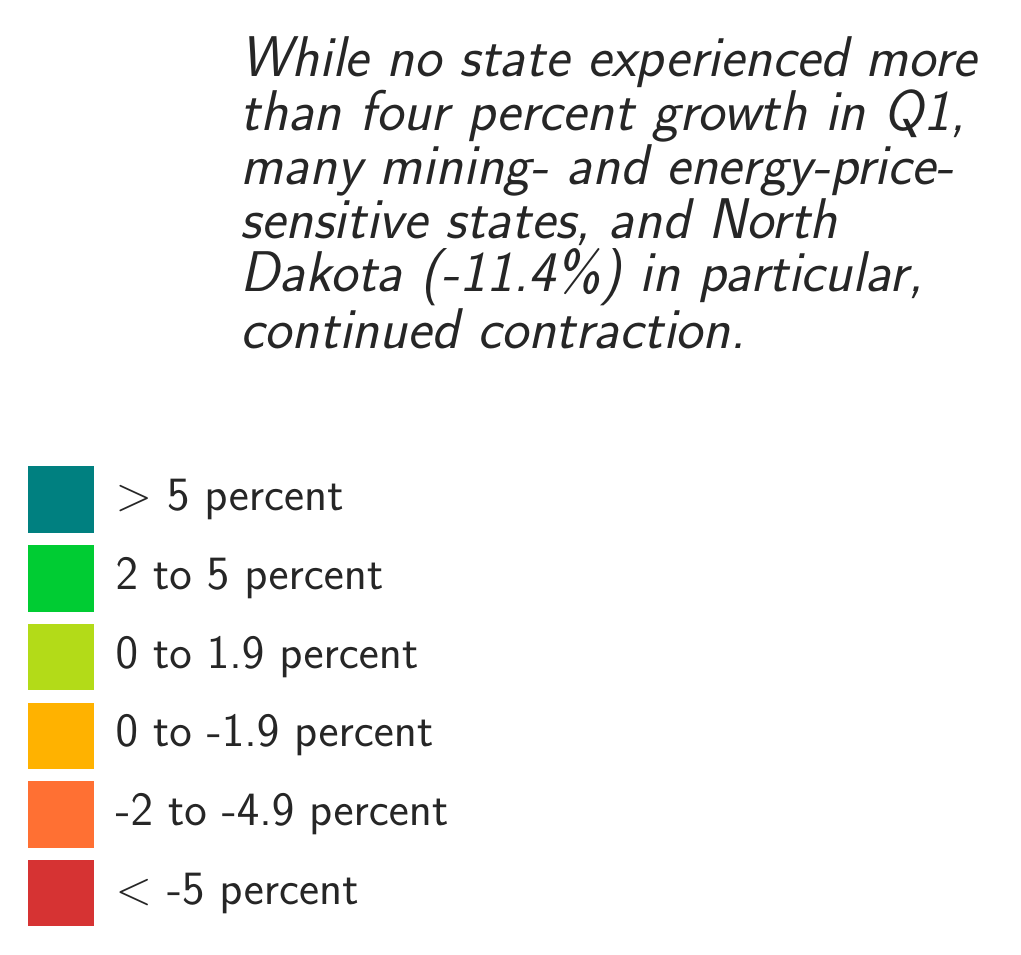
\begin{tikzpicture}
\USA[every state={draw=white, ultra thick, fill=black!10}]
\node[draw=none, minimum size=24pt,inner sep=0pt, fill=blue!50!green] at (25cm, -07cm)(C) {};
\node[right] at (C) {\LARGE \textcolor{black!85}{\quad $>$ 5 percent}};
\node[draw=none, minimum size=24pt,inner sep=0pt, fill=green!80!blue] at (25cm, -08cm)(A) {};
\node[right] at (A) {\LARGE \textcolor{black!85}{\quad 2 to 5 percent}};
\node[draw=none, minimum size=24pt,inner sep=0pt, fill=yellow!70!green] at (25cm, -09cm)(B) {};
\node[right] at (B) {\LARGE \textcolor{black!85}{\quad 0 to 1.9 percent}};
\node[draw=none, minimum size=24pt,inner sep=0pt, fill=orange!60!yellow] at (25cm, -10cm)(D) {};
\node[right] at (D) {\LARGE \textcolor{black!85}{\quad 0 to -1.9 percent}};
\node[draw=none, minimum size=24pt,inner sep=0pt, fill=red!40!orange!80] at (25cm, -11cm)(E) {};
\node[right] at (E) {\LARGE \textcolor{black!85}{\quad -2 to -4.9 percent}};
\node[draw=none, minimum size=24pt,inner sep=0pt, fill=red!80!black!80] at (25cm, -12cm)(F) {};
\node[right] at (F) {\LARGE \textcolor{black!85}{\quad $<$ -5 percent}};
\node[below, align=left, draw=none,fill=none] at (32cm, -1cm)(G) 
{\huge \textcolor{black!85}{\textsl{While no state experienced more}} \\ 
\huge \textcolor{black!85}{\textsl{than four percent growth in Q1, }}\\ 
\huge \textcolor{black!85}{\textsl{many mining- and energy-price-}}\\
\huge \textcolor{black!85}{\textsl{sensitive states, and North }}\\
\huge \textcolor{black!85}{\textsl{Dakota (-11.4\%) in particular, }}\\
\huge \textcolor{black!85}{\textsl{continued contraction.}}};
\end{tikzpicture}
}		
}
\vspace{1mm}

	% Footer
		\indent  {\footnotesize{Source: U.S. Bureau of Economic Analysis (BEA), \href{http://www.bea.gov/newsreleases/regional/gdp_state/qgsp_newsrelease.htm}{Regional Economic Accounts: GDP by State} 
	}

\end{document}